
\section{设计内容}

\subsection{概要设计}

系统环境:
\begin{enumerate}
\item Ubuntu 16.04
\item python 3.6
\item tensorflow 1.12.0
\end{enumerate}

\subsection{具体设计}

tcp\_newreno.py是newreno算法的Python移植,而tcp\_base.py表示着Deep Q-learning算法模型,我们小组先进行算法的转换,将C++转化为Python,与论文作对比,然后在TcpNewReno.py中实现强化学习的模型。
首先分析数据接收的对比图:

\begin{figure}[h]
	\centering
	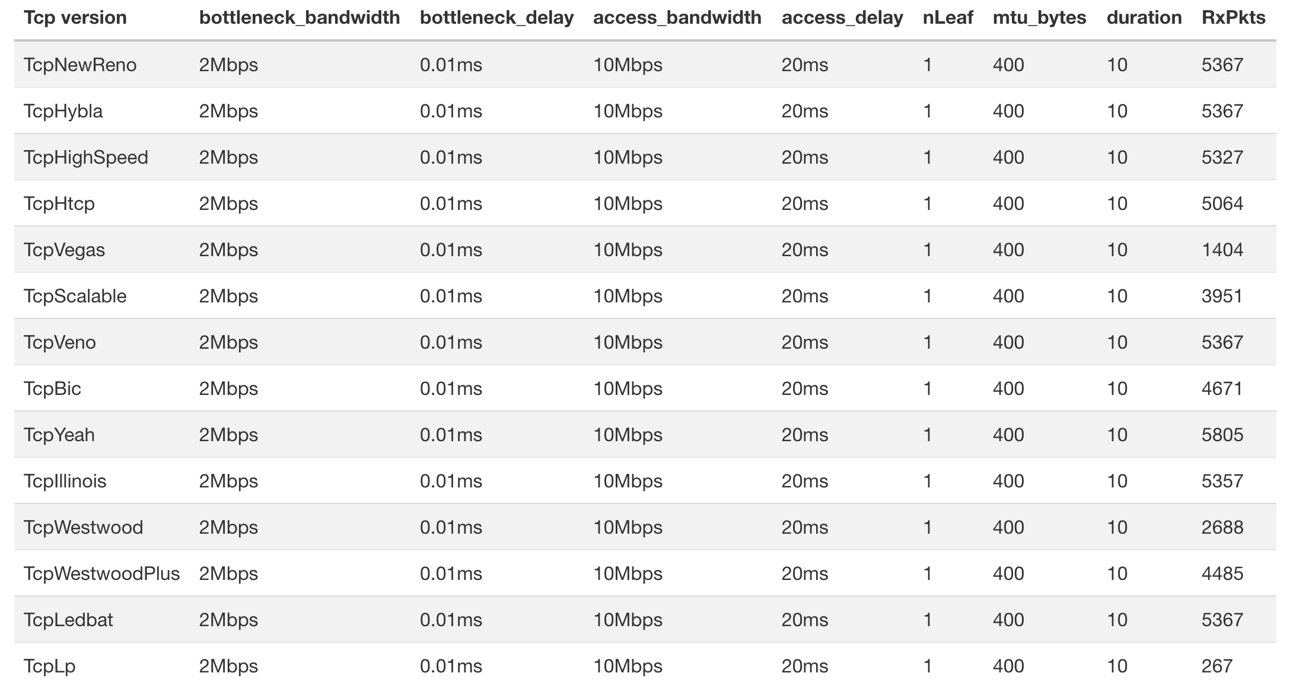
\includegraphics[width=0.8\linewidth]{figure/figure1.png}
	\caption{传统方法数据接收对比图}
	\label{figure1}
\end{figure}

由于要选择一个数据包接收效果尽可能好的协议,同时仿真智能体应基于时间,我们选择了TcpNewReno作为参照的仿真协议。通过这个协议可以得到传统方法的CWND图。

\begin{figure}[h]
	\centering
	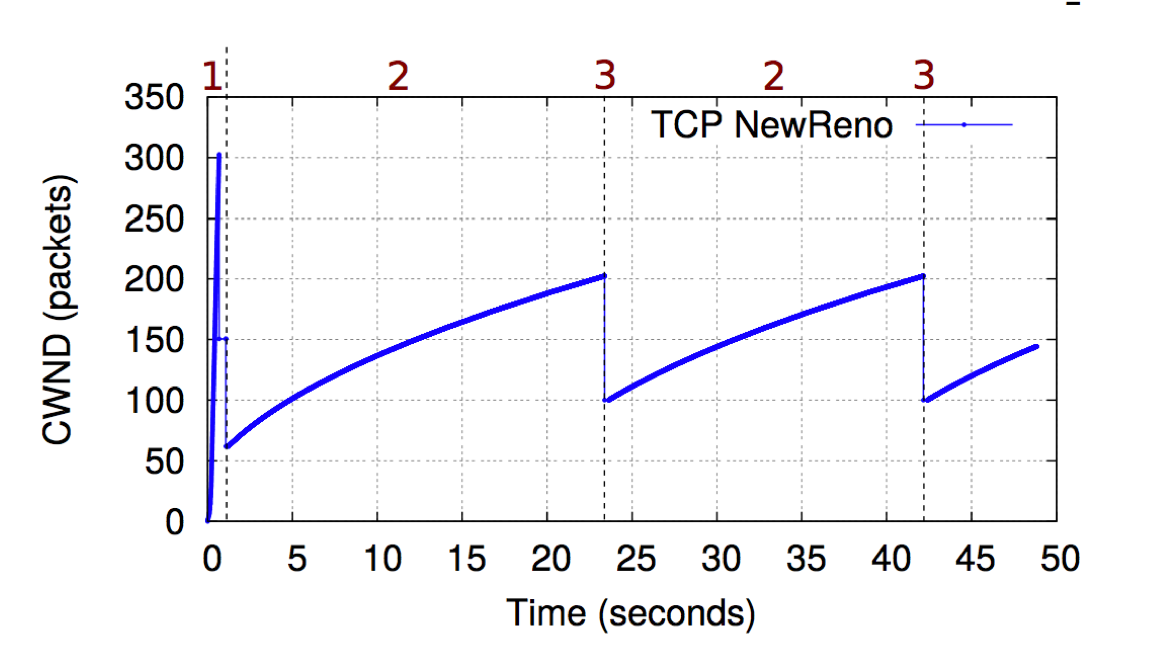
\includegraphics[width=0.6\linewidth]{figure/figure2.png}
	\caption{传统方法CWND曲线图}
	\label{figure2}
\end{figure}

对应着强化学习的方法,可以从QTCP论文之中获取吞吐量以及RTT的示意图。
接下来第一步,我们小组尝试改进论文中的DEMO,也就是自适应视频流传输的算法,尝试加快模型的收敛速度。
第二步,尝试传统方法从C++到Python的移植。
第三步,采用Deep Q-Learning算法进行训练,算法模型如下图。
第四步,改进reward和action。

\begin{figure}[htbp]
\centering
\begin{minipage}[t]{0.48\textwidth}
\centering
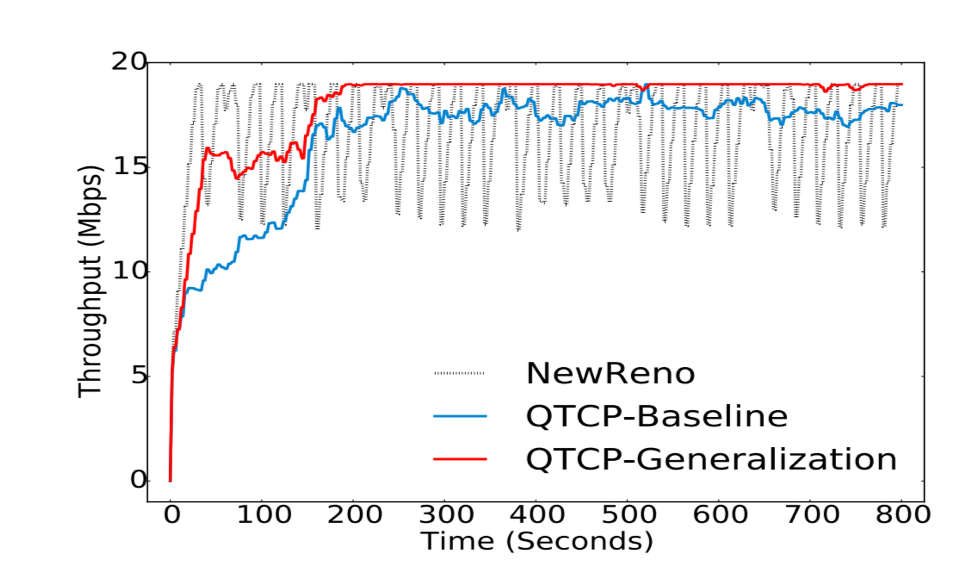
\includegraphics[width=6cm]{figure/figure3.png}
\caption{吞吐量}
\end{minipage}
\begin{minipage}[t]{0.48\textwidth}
\centering
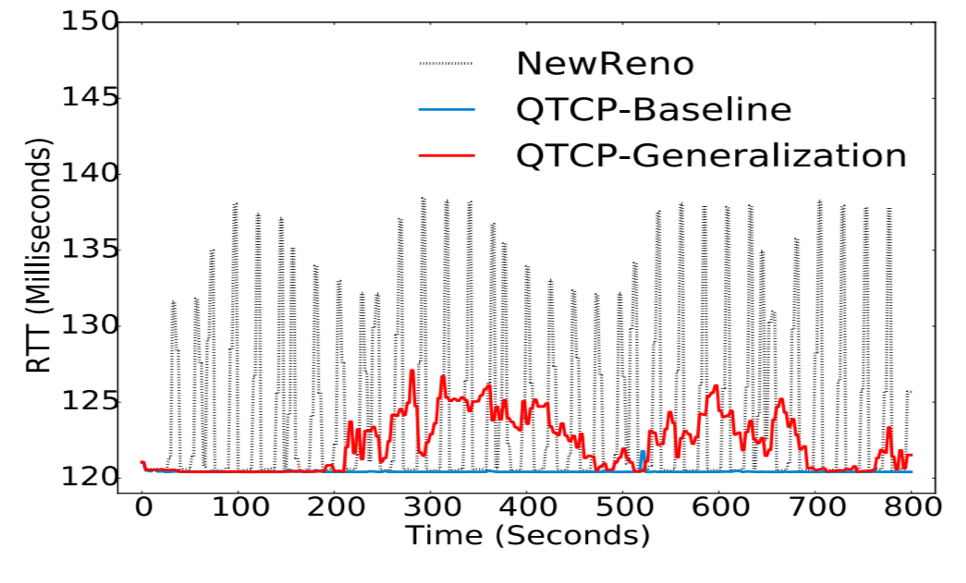
\includegraphics[width=6cm]{figure/figure4.png}
\caption{RTT}
\end{minipage}
\centering
	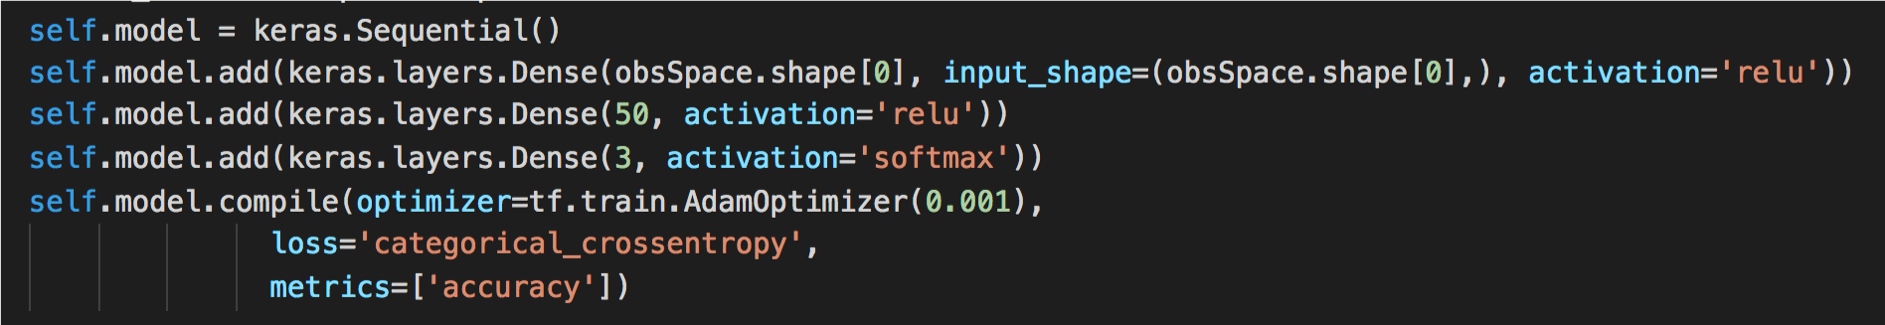
\includegraphics[width=0.8\linewidth]{figure/figure5.png}
	\caption{强化学习模型}
	\label{figure5}
\end{figure}